\documentclass[a4paper]{article}
\usepackage{reporter}
\usepackage{tabularx}
\usepackage{booktabs}
\usepackage{tikz}
\usetikzlibrary{patterns}

\newcommand{\QUE}[1]{\noindent\boxed{\textbf{Question}} \textit{#1}\newline}
\newcommand{\ANS}{\noindent\boxed{\textbf{Solution}}}
% \newcommand{\QUE}[1]{\noindent\boxed{\textbf{问 题}} \textit{#1}\newline}
% \newcommand{\ANS}{\noindent\boxed{\textbf{解 答}}}

\newcommand{\COM}[1]{\texttt{#1}}
\newcommand{\QED}{\hfill\(\square\)\newline\hrule\vspace{3mm}}
\newcommand{\END}{\vspace{3mm}\hrule\vspace{3mm}}


\newcommand{\TITLE}{Optics Lecture Answer}
\newcommand{\DISCR}{The project about the Physics and other. Write your Describution about the title.}
\newcommand{\EDITION}{Edition 1.0.0}
\newcommand{\AUTHOR}{Youpeng Wu}
\newcommand{\AUTHORS}{
Youpeng Wu\\
}
\newcommand{\CRDATES}{\textsc{September 9, 2025}}
\newcommand{\DATES}{\textsc{\today}}
\newcommand{\LOGO}{figure/logo.png}
\newcommand{\ANNOUNCE}{This work is licensed under a Creative Commons ``Attribution NonCommercial-ShareAlike 3.0 Unported'' license. }
\begin{document}
\HEADPAGE

\begin{center}
        \Large\textbf{\TITLE}\\
        \vspace*{3mm}
        \normalsize
        \AUTHOR
\end{center}
\vspace*{5mm}
\begin{abstract}
        This is a unofficial answer for optics lecture in PKU 2025 autumn. This is only for learning and communication. If you have any question, please contact me.
\end{abstract}

\tableofcontents
\newpage
%正文
\section{作业题目列表}

\begin{table}[htbp]
\caption{各章节题目编号}
\centering
\renewcommand{\arraystretch}{1.2}
\begin{tabularx}{\textwidth}{@{}l|X@{}}
\toprule
章节 & 题目编号 \\
\midrule
第二章 几何光学基本原理 & 2.5, 2.8, 2.10, 2.16 \\
\midrule
第三章 光波衍射的标量波理论 & 
第四节 圆孔、圆屏的费涅尔衍射:3.3, 3.4 \newline
第五节 半边无限大屏的费涅尔衍射:3.9 \newline
第六节 单缝、矩孔的夫琅禾费衍射:3.12 \newline
第七节 圆孔的夫琅禾费衍射:3.10, 3.11 \newline
第八节 其它形状孔的夫琅禾费衍射:3.17, 3.18 \\
\midrule
第四章 光波在介质界面的反射与折射 & 4.2, 4.3, 4.5, 4.6, 4.11 \\
\midrule
第五章 光波在晶体中的传播 & 
第二节 光线速度与相速度:5.1, 5.2 \newline
第三节 晶体双折射:5.7 \newline
第四节 晶体光学器件:5.4, 5.5, 5.9 \newline
第五节 旋光:5.10, 5.11 \\
\midrule
第六章 光场的空间相干性 & 6.1, 6.2, 6.6, 6.7, 6.9, 6.10 \\
\midrule
第七章 光场的时间相干性 & 7.3, 7.5, 7.7, 7.9 \\
\midrule
第八章 光场的偏振态 & 8.2, 8.7, 8.8, 8.11 \\
\midrule
第九章 成像系统 & 
第一节 几种基本成像系统:9.1, 9.2, 9.7, 9.9 \newline
第二节 望远镜:9.21, 9.25 \\
\midrule
第十章 干涉装置 & 
第一节 分波前装置:10.1, 10.2, 10.3, 10.6 \newline
第二节 薄膜干涉:10.11, 10.12, 10.13, 10.17 \newline
第三节 多光束干涉与法布里-珀罗干涉仪:10.19, 10.20 \newline
第四节 偏振光干涉:10.22 \newline
第五节 李奥滤光器:10.23 \\
\midrule
第十一章 衍射光栅 & 
第一节 光栅及其夫琅禾费衍射场:11.2, 11.4, 11.7 \newline
第二节 光栅光谱仪:11.10 \\
\bottomrule
\end{tabularx}
\end{table}
\newpage

\section{第二章答案}

\QUE{2.5 试用费马原理证明通过旋转双曲面一个焦点的光线经旋转双曲面反射后,其反射延长线经过另一个焦点}

\ANS 

要证明这个问题,由费马定理:光在两点间传播时,总是沿着光程为最小值的路径传播。我们构造这样一个证明: 对于从焦点 \(F_1\) 出发,经过旋转双曲面在点\(P\)反射后到达\(Q\)的光程, 在\(QP\)的延长线经过另一个焦点\(F_2\)时取得最小值。

对于双曲面上的点\(P\), 有关系
\[
|PF_2|-|PF_1|=2a \to |PF_1|=|PF_2|-2a
\]
而光程为
\[
L=|PF_1|+|PQ|=|PF_2|+|PQ| -2a
\]
当光程取最小时, \(L\) 取最小值, 则此时\(P\), \(Q\), \(F_2\) 三点共线, 即光线的反射延长线经过另一个焦点\(F_2\).

\QED

\QUE{2.8 光线以入射角\(i\)从折射率为\(n_w\)的水中入射到折射率为\(n\)厚度为\(h\)的玻璃中, 玻璃的折射率大于水的折射率. 计算光线在玻璃中的光程\(L\)}

\ANS

进入玻璃后, 光线的折射角为:
\[
n \sin r = n_w \sin i \to \sin r = \frac{n_w}{n} \sin i
\]
设光线在玻璃中的传播距离为\(d\), 则有:
\[
h = d \cos r \to d = \frac{h}{\cos r} = \frac{h}{\sqrt{1-\sin^2 r}} = \frac{h}{\sqrt{1-\left(\frac{n_w}{n}\sin i\right)^2}}
\]
光程为:
\[
L = n d = \frac{n h}{\sqrt{1-\left(\frac{n_w}{n}\sin i\right)^2}}= \frac{n^2 h}{\sqrt{n^2 - n_w^2 \sin^2 i}}
\]

\END

\QUE{2.10 光线经折射率为\(n\)的球形水珠折射. 求折射后光线偏向角的最大值}

\ANS

光线进入水珠后会发生两次折射, 设入射角为\(\alpha\), 折射角为\(\beta\). 则有:
\[
\sin \alpha = n \sin \beta \to \beta = \arcsin \frac{\sin \alpha}{n}
\]
光线偏向角\(\theta\)为:
\[
\theta = 2(\alpha - \beta) = 2\alpha - 2 \arcsin \frac{\sin \alpha}{n}
\]
对\(\alpha\)求导:
\[
\frac{d\theta}{d\alpha} = 2 - \frac{2 \cos \alpha}{n \sqrt{1-\left(\frac{\sin \alpha}{n}\right)^2}} = 0
\to 2 = \frac{2 \cos \alpha}{n \sqrt{1-\left(\frac{\sin \alpha}{n}\right)^2}}
\to n \sqrt{1-\left(\frac{\sin \alpha}{n}\right)^2} =  \cos \alpha
\]
当\(\alpha=\pi/2\)时, \(\theta\) 取得最大值:
\[
\theta_{max} = \pi - 2 \arcsin \frac{1}{n}
\]

\begin{minipage}[c]{0.4\textwidth}
    \centering
    


% Pattern Info
 
\tikzset{
pattern size/.store in=\mcSize, 
pattern size = 5pt,
pattern thickness/.store in=\mcThickness, 
pattern thickness = 0.3pt,
pattern radius/.store in=\mcRadius, 
pattern radius = 1pt}
\makeatletter
\pgfutil@ifundefined{pgf@pattern@name@_6mh2pgkdc}{
\makeatletter
\pgfdeclarepatternformonly[\mcRadius,\mcThickness,\mcSize]{_6mh2pgkdc}
{\pgfpoint{-0.5*\mcSize}{-0.5*\mcSize}}
{\pgfpoint{0.5*\mcSize}{0.5*\mcSize}}
{\pgfpoint{\mcSize}{\mcSize}}
{
\pgfsetcolor{\tikz@pattern@color}
\pgfsetlinewidth{\mcThickness}
\pgfpathcircle\pgfpointorigin{\mcRadius}
\pgfusepath{stroke}
}}
\makeatother
\tikzset{every picture/.style={line width=0.75pt}} %set default line width to 0.75pt        

\begin{tikzpicture}[x=0.75pt,y=0.75pt,yscale=-1,xscale=1]
%uncomment if require: \path (0,300); %set diagram left start at 0, and has height of 300

%Shape: Circle [id:dp47523115765045854] 
\draw  [pattern=_6mh2pgkdc,pattern size=12pt,pattern thickness=0.75pt,pattern radius=0.75pt, pattern color={rgb, 255:red, 155; green, 155; blue, 155}] (66.67,148.33) .. controls (66.67,104.89) and (101.89,69.67) .. (145.33,69.67) .. controls (188.78,69.67) and (224,104.89) .. (224,148.33) .. controls (224,191.78) and (188.78,227) .. (145.33,227) .. controls (101.89,227) and (66.67,191.78) .. (66.67,148.33) -- cycle ;
%Straight Lines [id:da7610905084348585] 
\draw  [dash pattern={on 4.5pt off 4.5pt}]  (145.33,148.33) -- (240.26,58.18) ;
%Straight Lines [id:da26122017173896583] 
\draw    (202.67,93.88) -- (212.67,188.55) ;
\draw [shift={(206.99,134.75)}, rotate = 83.97] [fill={rgb, 255:red, 0; green, 0; blue, 0 }  ][line width=0.08]  [draw opacity=0] (8.93,-4.29) -- (0,0) -- (8.93,4.29) -- cycle    ;
%Straight Lines [id:da08455822982829975] 
\draw  [dash pattern={on 4.5pt off 4.5pt}]  (202.67,93.88) -- (107.34,79.22) ;
\draw [shift={(150.06,85.79)}, rotate = 8.75] [fill={rgb, 255:red, 0; green, 0; blue, 0 }  ][line width=0.08]  [draw opacity=0] (8.93,-4.29) -- (0,0) -- (8.93,4.29) -- cycle    ;
%Straight Lines [id:da5652093586635702] 
\draw  [dash pattern={on 4.5pt off 4.5pt}]  (145.33,148.33) -- (248.3,209.83) ;
%Shape: Arc [id:dp4615412617607718] 
\draw  [draw opacity=0] (204.48,107.76) .. controls (203.89,107.84) and (203.28,107.88) .. (202.67,107.88) .. controls (198.62,107.88) and (194.99,105.99) .. (192.55,103) -- (202.67,93.88) -- cycle ; \draw   (204.48,107.76) .. controls (203.89,107.84) and (203.28,107.88) .. (202.67,107.88) .. controls (198.62,107.88) and (194.99,105.99) .. (192.55,103) ;  
%Shape: Arc [id:dp06900445719233972] 
\draw  [draw opacity=0] (200.37,181.88) .. controls (200.65,181.35) and (200.97,180.84) .. (201.33,180.34) .. controls (203.7,177.06) and (207.37,175.23) .. (211.22,175.01) -- (212.67,188.55) -- cycle ; \draw   (200.37,181.88) .. controls (200.65,181.35) and (200.97,180.84) .. (201.33,180.34) .. controls (203.7,177.06) and (207.37,175.23) .. (211.22,175.01) ;  
%Straight Lines [id:da8096367973292018] 
\draw    (212.67,188.55) -- (168.67,257.22) ;
\draw [shift={(194.18,217.41)}, rotate = 122.65] [fill={rgb, 255:red, 0; green, 0; blue, 0 }  ][line width=0.08]  [draw opacity=0] (8.93,-4.29) -- (0,0) -- (8.93,4.29) -- cycle    ;
%Straight Lines [id:da777128522091038] 
\draw    (202.67,93.88) -- (140.67,37.22) ;
\draw [shift={(167.98,62.18)}, rotate = 42.43] [fill={rgb, 255:red, 0; green, 0; blue, 0 }  ][line width=0.08]  [draw opacity=0] (8.93,-4.29) -- (0,0) -- (8.93,4.29) -- cycle    ;
%Shape: Arc [id:dp8738118911332267] 
\draw  [draw opacity=0] (224.39,195.71) .. controls (222.92,198.4) and (220.56,200.56) .. (217.53,201.68) .. controls (213.73,203.09) and (209.67,202.57) .. (206.34,200.61) -- (212.67,188.55) -- cycle ; \draw   (224.39,195.71) .. controls (222.92,198.4) and (220.56,200.56) .. (217.53,201.68) .. controls (213.73,203.09) and (209.67,202.57) .. (206.34,200.61) ;  
%Shape: Arc [id:dp5289496782411189] 
\draw  [draw opacity=0] (193.1,104.09) .. controls (192.66,103.69) and (192.25,103.25) .. (191.86,102.78) .. controls (189.28,99.65) and (188.44,95.64) .. (189.2,91.85) -- (202.67,93.88) -- cycle ; \draw   (193.1,104.09) .. controls (192.66,103.69) and (192.25,103.25) .. (191.86,102.78) .. controls (189.28,99.65) and (188.44,95.64) .. (189.2,91.85) ;  
%Shape: Arc [id:dp34734335147134476] 
\draw  [draw opacity=0] (193.16,83.98) .. controls (195.26,81.76) and (198.09,80.27) .. (201.31,79.95) .. controls (205.34,79.56) and (209.13,81.09) .. (211.86,83.83) -- (202.67,93.88) -- cycle ; \draw   (193.16,83.98) .. controls (195.26,81.76) and (198.09,80.27) .. (201.31,79.95) .. controls (205.34,79.56) and (209.13,81.09) .. (211.86,83.83) ;  

% Text Node
\draw (212.67,203.73) node [anchor=north west][inner sep=0.75pt]    {$\alpha $};
% Text Node
\draw (192,159.07) node [anchor=north west][inner sep=0.75pt]    {$\beta $};
% Text Node
\draw (190,109.73) node [anchor=north west][inner sep=0.75pt]    {$\beta $};
% Text Node
\draw (200,60.4) node [anchor=north west][inner sep=0.75pt]    {$\alpha $};
% Text Node
\draw (168.67,95.07) node [anchor=north west][inner sep=0.75pt]    {$\beta $};
% Text Node
\draw (228.67,174.4) node [anchor=north west][inner sep=0.75pt]    {$P_{1}$};
% Text Node
\draw (217.33,87.73) node [anchor=north west][inner sep=0.75pt]    {$P_{2}$};


\end{tikzpicture}

\end{minipage}
\begin{minipage}[c]{0.55\textwidth}
\textbf{球内多次反射}\newline
\COM{
如图所示, 在入射光线-球心平面上, 光线入射角为\(\alpha\), 折射角为\(\beta\). 当入射光线掠射入射时(沿切线方向), 入射角\(\alpha = \frac{\pi}{2}\), 此时折射角达到其最大值\(\beta_{max}=\arcsin \frac{1}{n}\), 即全反射角. 由于球的性质, 光线在球内的入射角也为\(\beta < \beta_{max}\).  所以对于一个理想的球形, 不会发生全反射, 此时光线射出. 从对称性的角度考虑会更加容易. \newline
但是如果不在几何光学的条件下, 在小于全反射角的入射角下, 还是有部分光线会发生反射, 这时就会有多次反射的情况发生.
}
\end{minipage}

\END

\QUE{2.16 一个透明圆柱由厚度均匀的多层介质构成,各层介质均为圆筒状。已知由内向外各层介质的折射率和内半径分别为 \(n_l\) 和 \(r_l\),其中 \(l=1,2,\ldots,m\),光线在透明圆柱的截面内。求光线在各界面上的折射角 \(i_l\) 之间的关系。}

\ANS

光线在各层介质中的传播满足光线微分方程:
\[
\frac{d^2 \vec{r}}{d\tau^2}=n\nabla n
\]
由于这是一个柱对称的系统, 所以满足角动量守恒, 定义质量为1的粒子在各层介质中的角动量为:
\[
n_lr_l \sin i_l = \text{Const.} \quad (l=1,2,\ldots,m)
\]
所以此时:
\[
n_l r_l \sin i_l = n_k r_k \sin i_k = \text{Const.} \quad (l,k=1,2,\ldots,m)
\]

\section{第三章答案}

\QUE{3.3 一列光强为 \(I_0\),波长为 \(589.3\,\mathrm{nm}\) 的平面单色光波垂直入射到衍射屏上,衍射屏的透光部分为一个内直径等于 \(0.5\,\mathrm{mm}\),外直径等于 \(1.0\,\mathrm{mm}\) 的圆环。求距衍射屏 \(50\,\mathrm{cm}\) 处光轴上的光强。}

\ANS 



\begin{figure}
        \centering
        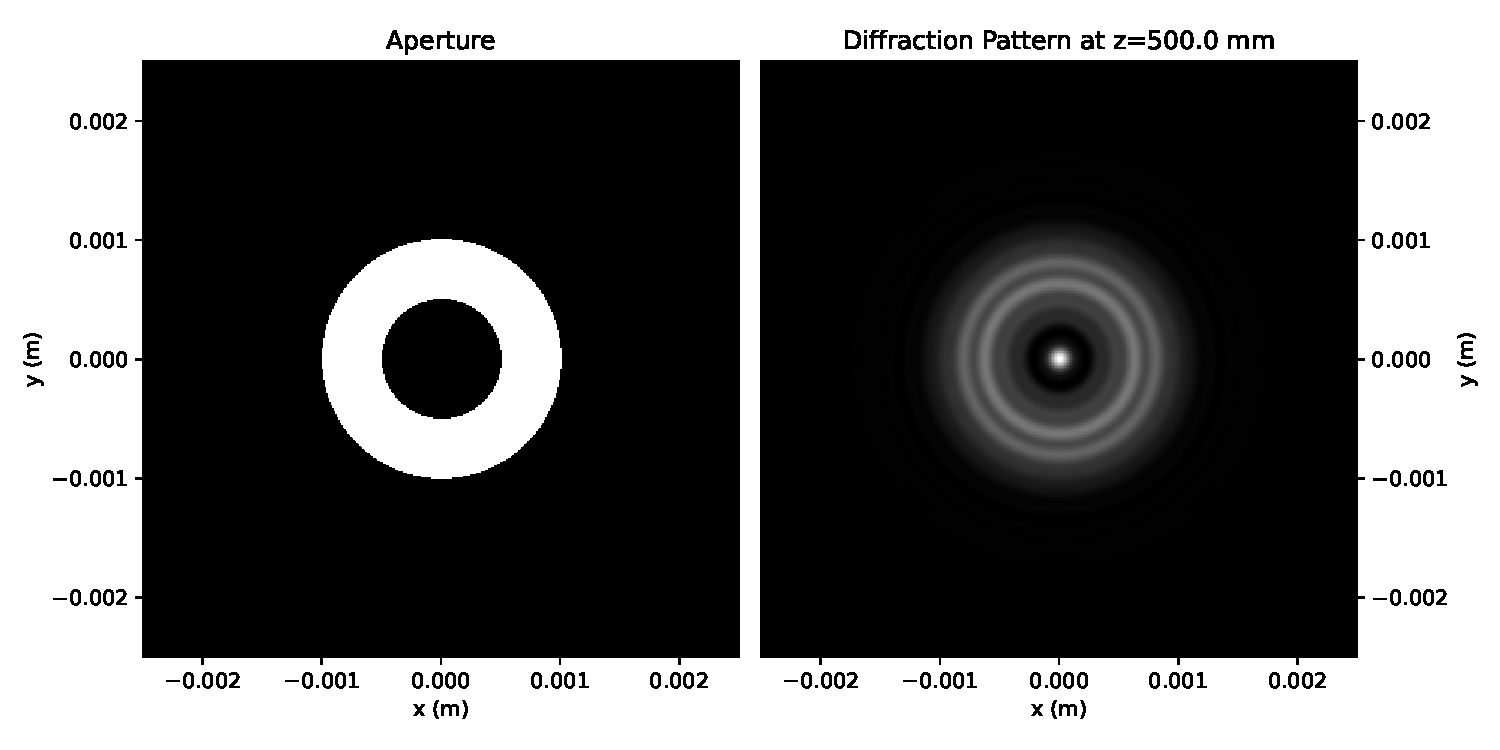
\includegraphics[width=0.6\textwidth]{figure/q3_3_diffraction_pattern.pdf}
        \caption{圆环衍射光强分布}
        \label{fig:q3_3_diffraction_pattern}
\end{figure}

\END 

\QUE{3.4 用波长为 \(632.8\,\mathrm{nm}\) 的平面单色光波垂直照射衍射屏,衍射屏的透光部分为一个圆孔。已知在衍射屏后方距衍射屏 \(2.0\,\mathrm{m}\)、\(1.0\,\mathrm{m}\)、\(0.67\,\mathrm{m}\)、\(0.50\,\mathrm{m}\)、\(0.40\,\mathrm{m}\) 等处光轴上的光强为 0。求圆孔的直径。}

\QUE{3.9 波长为 \(650\,\mathrm{nm}\) 的平行光照射到一个刀片上。求刀片后方 \(20\,\mathrm{cm}\) 处的接收屏上最大光强出现的位置到刀片边缘几何投影的距离。}

\QUE{3.10 光强为 \(I_0\),波长为 \(\lambda\) 的平行光正入射到一个衍射屏上,衍射屏的透光部分是一个半径为 \(d\) 的圆孔,圆孔中嵌有折射率为 \(n\) 的玻璃,玻璃的背面刻有深度为 \(h\)、直径为 \(d\) 的浅槽。求衍射屏后方光轴上距衍射屏 \(b\) 处的光强,距离 \(b\) 满足条件 \(b^2 \gg d^2\)。}

\QUE{3.11 实验室里光导轨长 \(2\,\mathrm{m}\)。用氦氖激光演示圆孔夫琅禾费衍射。求合适的圆孔直径。}

\QUE{3.12 使波长为 \(589.3\,\mathrm{nm}\) 的平行光正入射到宽度为 \(0.10\,\mathrm{mm}\) 的狭缝上,接收屏到狭缝距离为 \(2.0\,\mathrm{m}\)。求接收屏上零级衍射斑的宽度。}

\QUE{3.17 在一个夫琅禾费衍射装置中,接收透镜的焦距为 \(F\),光源的波长为 \(\lambda\),衍射屏上的开孔为两个对角线长度分别为 \(a\) 和 \(b\) 的菱形,求衍射场的光强分布。}

\QUE{3.18 在一个夫琅禾费衍射装置中,接收透镜的焦距为 \(F\),光源的波长为 \(\lambda\),衍射屏上的开孔为长短半轴分别为 \(a\) 和 \(b\) 的椭圆,求衍射场的光强分布。}


\end{document}
